
\section{Filtro pasa-bajos pasivo}

\quad \quad En esta secci\'on dise\~naremos y analizaremos el comportamiento de un filtro RC de primer orden pasa-bajos.

\subsection{Dise\~no}
\quad \quad Seg\'un el n\'umero de grupo asignado fijamos la frecuencia de corte del filtro en $16kHz$. Luego calculamos la funci\'on transferencia del mismo obteniendo

\begin{equation}\label{ganancia_2}
H(s) = \frac{1}{sCR+1}
\end{equation}

Donde la frecuencia de corte $f_{0}$ vale

\begin{equation}\label{freccorte_2}
f_{0} = 2\pi CR
\end{equation}

Dado que los valores de ambos componentes son comerciales y estandarizados, seleccionamos un par para los cuales creemos que el error es lo suficientemente peque\~no. As\'i, fijamos $C=10nF$ y $R=1k\Omega$ con lo cual la frecuencia de corte te\'orica es $f_{0}=15915,49Hz$.

\subsection{Se\~nal cuadrada}

\quad \quad Una vez seleccionados los componentes se arm\'o el circuito y se lo someti\'o a una se\~nal cuadrada (cuyo valor medio es nulo) de $10V_{pp}$ a una frecuencia dada de $8kHz$ con la siguiente respuesta medida en osciloscopio.

\begin{figure}[H]
    \centering
    \includegraphics[width=0.9\textwidth]{./EJ2/EJ2_respuesta_a_cuadrada.png}
    \caption{Respuesta a una se\~nal cuadrada}
    \label{fig:rtacuad_2} 
\end{figure}

\quad \quad En la figura \ref{fig:rtacuad_2} se puede observar una forma curva en los flancos ascendentes y descendientes de la respuesta del sistema a la se\~nal cuadrada (curva resaltada en celeste). Esto se debe principalmente a los intervalos de carga y descarga del capacitor, ante la inversi\'on de polaridad en sus bornes, obteniendo ese efecto de $"suavizaci\'on"$. Adem\'as, desde el punto de vista espectral podemos apreciar una atenuaci\'on en los arm\'onicos altos que componen la se\~nal cuadrada, debido a que esta entrada est\'a pasando por un filtro pasa-bajos. Esto tambi\'en contribuye a la distorsi\'on en la forma de la se\~nal.

\subsection{Respuesta en frecuencia}

\quad \quad Para confeccionar la respuesta en frecuencia del filtro se realiz\'o un barrido en frecuencia de la entrada, midiendo a la salida la relaci\'on entre la amplitud respecto a la de la entrada, y la fase. Luego se volcaron esos datos a una hoja de c\'alculo y se obtuvieron dos gr\'aficos que representan cada una de esas caracter\'isticas.

%\begin{figure}[H]
 %   \centering
 %   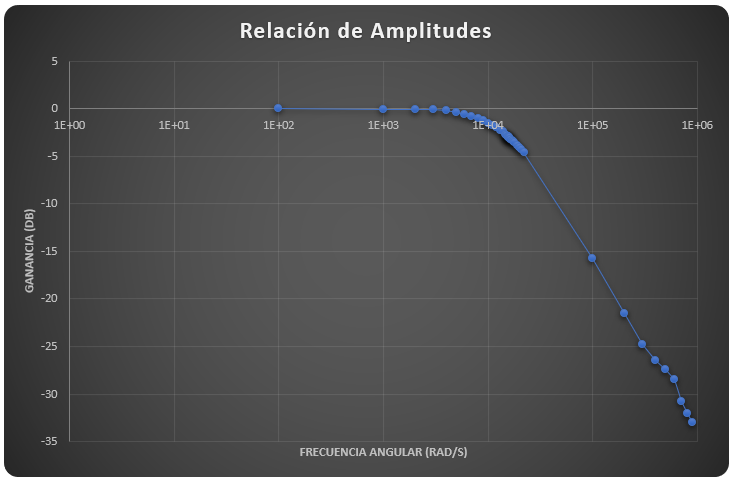
\includegraphics[width=0.9\textwidth]{./EJ2/EJ2_BODE_amp_medido.png}
 %   \caption{Diagrama BODE de amplitud medido}
 %   \label{fig: bode_amp_medido_2} 
%\end{figure}


%\begin{figure}[H]
 %   \centering
 %   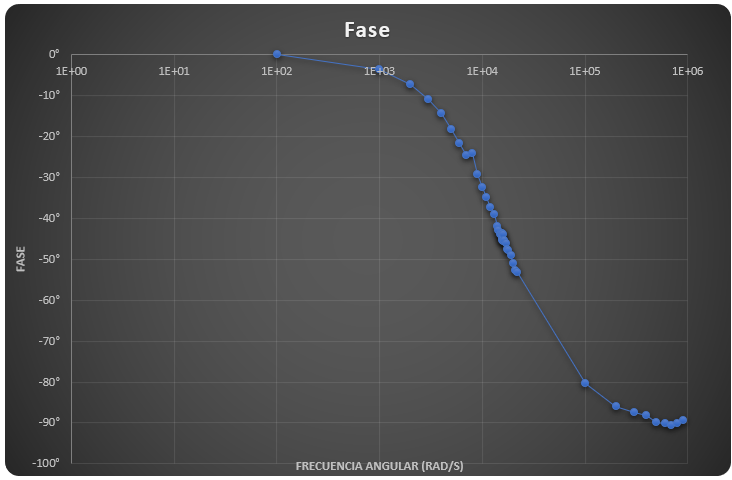
\includegraphics[width=0.9\textwidth]{./EJ2/EJ2_BODE_fase_medido.png}
 %   \caption{Diagrama BODE de fase medido}
 %   \label{fig: bode_fase_medido_2} 
%\end{figure}

\quad \quad La frecuencia de corte $"real"$ del circuito fue obtenida usando el osciloscopio, variando la frecuencia hasta encontrar un desfasaje de $-45^\circ$ en la salida respecto a la entrada. Seg\'un la figura \ref{fig:phase_2}, en este caso $f_{0}=15,57kHz$


\begin{figure}[H]
    \centering
    \includegraphics[width=0.9\textwidth]{./EJ2/EJ2_fase_osc.png}
    \caption{Medici\'on de frecuencia de corte}
    \label{fig:phase_2} 
\end{figure}
\quad \quad Adem\'as, se puede ver que el diagrama de BODE resultante de las mediciones es compatible con el an\'alisis te\'orico sobre el filtro.

\quad \quad Por otro lado, se desarroll\'o en serie de Fourier la se\~nal de entrada con el fin de encontrar las componentes de frecuencia que componen a dicha se\~nal. Usando los coeficientes de Fourier podemos observar la presencia de cada uno de los arm\'onicos (son todos impares), y se superpuso esta informaci\'on con el gr\'afico de amplitud del diagrama de BODE teórico. De esta forma, y calculando la funci\'on transferencia para sucesivos arm\'onicos, se observa que a frecuencias altas la baja amplitud de los arm\'onicos combinado con el bajo valor de la funci\'on transferencia nos permiten despreciar la presencia de dichos arm\'onicos.

\begin{figure}[H]
    \centering
    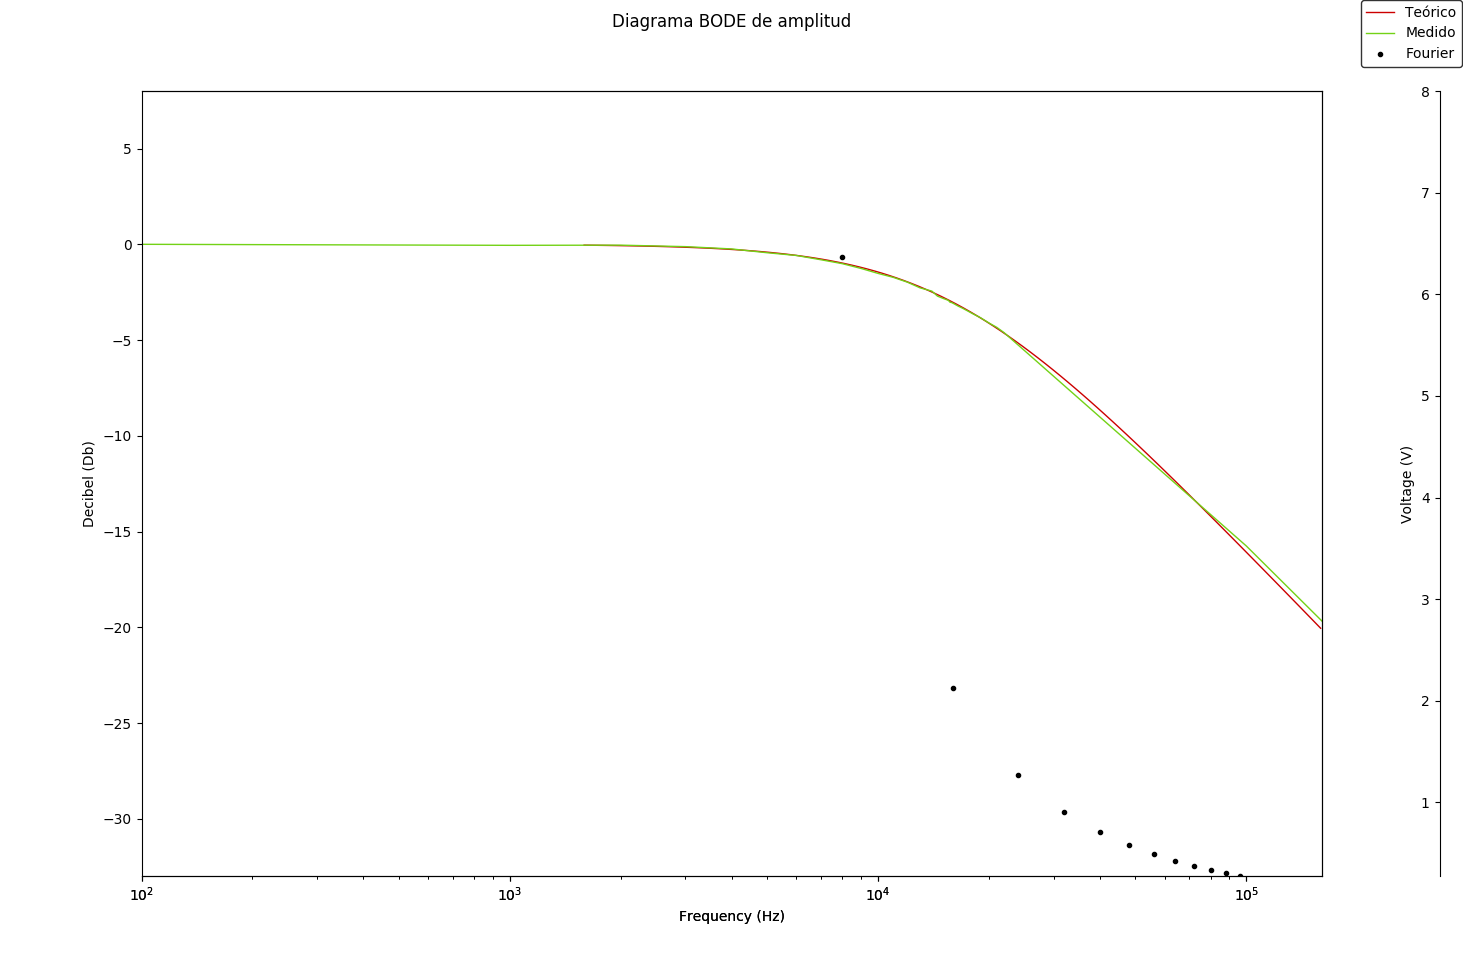
\includegraphics[width=0.9\textwidth]{./EJ2/EJ2_BODE_teorico.png}
    \caption{Diagrama BODE de amplitud te\'orico y medido y amplitud de arm\'onicos de entrada}
    \label{fig:bode_amp_superp_2} 
\end{figure}

\begin{figure}[H]
    \centering
    \includegraphics[width=0.9\textwidth]{./EJ2/EJ2_fase_BODE.png}
    \caption{Diagrama BODE de fase te\'orico y medido}
    \label{fig:bode_phase_superp_2} 
\end{figure}

\subsection{Comportamiento en alta frecuencia}

\quad \quad Si sometemos el circuito a una frecuencia moderadamente alta comparada con la frecuencia de corte del mismo, podemos ver que la funci\'on transferencia tiende a 
\begin{equation}\label{integrador_2}
    H(s)=\frac{1}{s}
\end{equation}

Lo que en transformada de Laplace implicar\'ia la integraci\'on de la se\~nal de entrada. Para comprobar esto forzamos al circuito en la pr\'actica a una frecuencia $f=250kHz$ seg\'un la figura \ref{fig:altafrec_2}. De este gr\'afico podemos resaltar que la se\~nal cuadrada de entrada resulta en una se\~nal de tipo triangular en la salida, confirmando la suposici\'on te\'orica planteada anteriormente.

\begin{figure}[H]
    \centering
    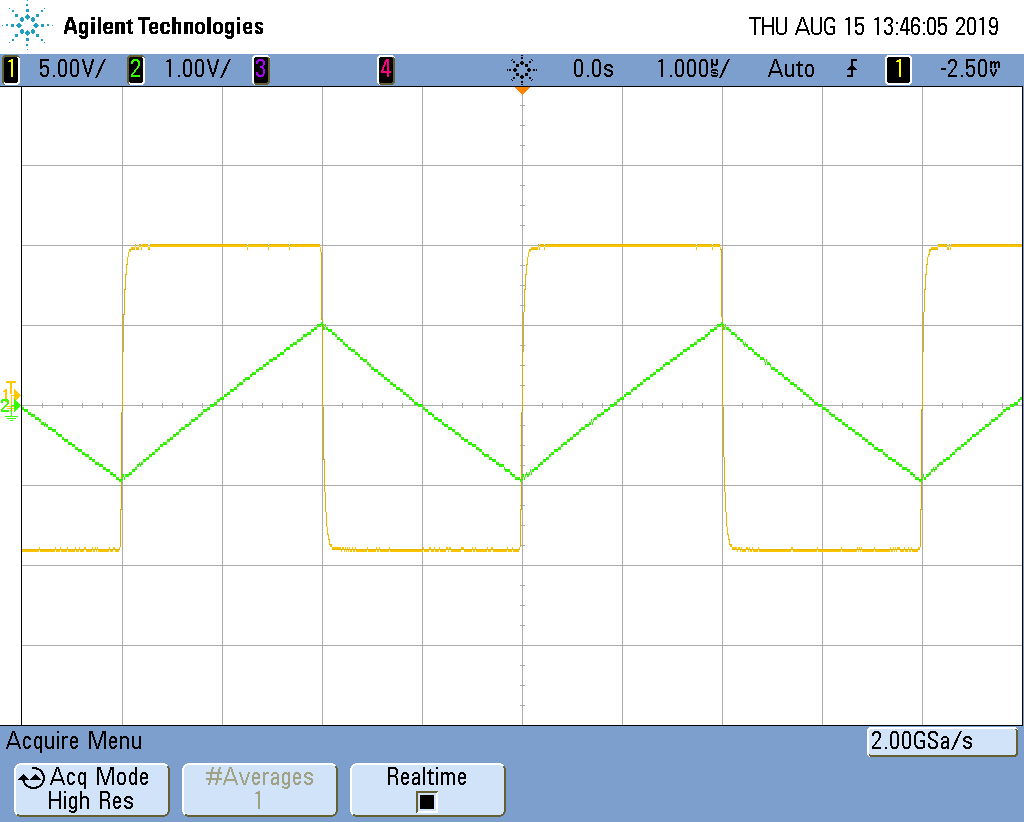
\includegraphics[width=0.9\textwidth]{./EJ2/EJ2_integrador.png}
    \caption{Respuesta a 250kHz}
    \label{fig:altafrec_2} 
\end{figure}

\quad \quad Si ahora probamos una frecuencia mucho mayor (en este caso $10MHz$) observamos una atenuaci\'on de la se\~nal de salida considerable, lo que produce que la salida sea susceptible de ser afectada por el ruido, como se puede ver en la figura \ref{fig:noise_2}.
 
 \begin{figure}[H]
    \centering
    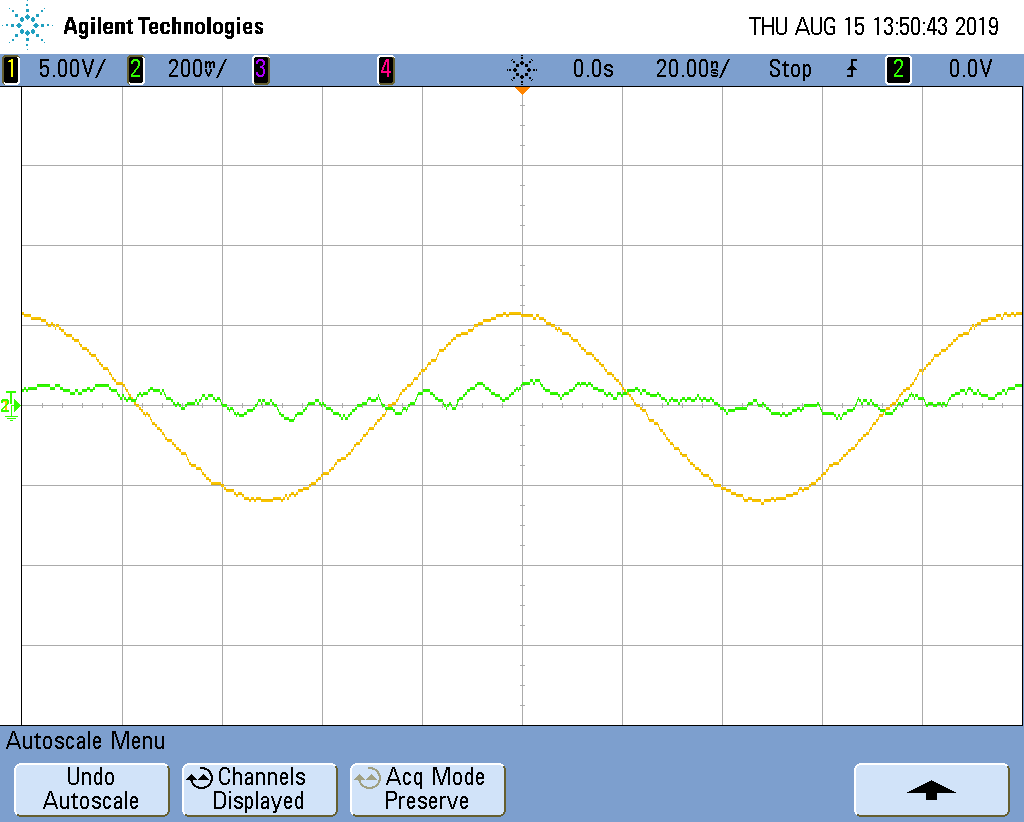
\includegraphics[width=0.9\textwidth]{./EJ2/EJ2_rta_alta_frec.png}
    \caption{Respuesta a 10MHz}
    \label{fig:noise_2}
\end{figure}
 
\subsection{Respuesta a $160Hz$}

\quad \quad Se conect\'o la entrada del circuito a una se\~nal cuadrada de similares caracter\'isticas que la primera, pero esta vez a una frecuencia de $160Hz$. Se midi\'o con osciloscopio la respuesta del circuito y se obtuvo la figura \ref{fig:160hz_2}. En ella podemos observar una atenuaci\'on casi nula de la salida (representada en color celeste) respecto de la entrada, asi como una fase pr\'acticamente nula. Esto se condice con el an\'alisis te\'orico que se puede realizar, dado que el t\'ermino que involucra a la frecuencia en la ecuaci\'on \ref{ganancia_2} se vuelve despreciable, con lo cual la funci\'on transferencia tiende al valor unitario.

\begin{figure}[H]
    \centering
    \includegraphics[width=0.9\textwidth]{./EJ2/EJ2_rta_160hz.png}
    \caption{Respuesta a $160Hz$}
    \label{fig:160hz_2} 
\end{figure}

